\documentclass{article}
\usepackage{graphicx} % Required for inserting images
\usepackage{titlesec}
\usepackage{listings}
\usepackage{enumitem}
\usepackage[top=1in, bottom=1in, left=1.25in, right=1.25in]{geometry}
\usepackage{amsmath}
\usepackage{tikz}
% Configure section numbering
\renewcommand{\thesection}{Part \Alph{section}}
\renewcommand{\thesubsection}{\arabic{subsection}:}
\renewcommand{\thesubsubsection}{(\alph{subsubsection})}

% Adjust section format
\titleformat{\section}{\normalfont\Large\bfseries}{\thesection}{1em}{}
\titleformat{\subsection}{\normalfont\large\bfseries}{\thesubsection}{1em}{}
\titleformat{\subsubsection}{\normalfont\normalsize\bfseries}{\thesubsubsection}{1em}{}


\title{\textbf{COL759 Assignment 1}}
\author{Anshik Sahu (2021CS10577)}
\date{August 2023}

\begin{document}

\maketitle
\section{}
\subsection{Perfect Two-time Security}
\subsubsection{}
Let the Adversary be defined as follows:
\begin{itemize}
    \item A gives (m0,m0) and (m1,m2) to the Challenger and receives (ct0,ct1), where m1 and m2 are distinct.
    \item If ct0 equals ct1, it guesses 0 else it guesses from {0,1} uniformly.
\end{itemize}
If the Encryption is not randomized,
\begin{itemize}
    \item if b=0, ct0=Enc(k,m0)=ct1. Hence b'=0.
    \item if b=1, ct0 and ct1 are distinct due to the correctness of the encryption. hence b'=0 or 1 with equal probability.
\end{itemize}
Thus, for a non randomized encryption,
\[Pr_{k}[A \text{ winning } \epsilon \text{-perfect two-time security game}] = \frac{1}{2} + \frac{1}{2} \cdot \frac{1}{2} = \frac{3}{4}
\]
Hence, a non randomized encryption is not perfect two-time secure.\\
For a randomized encryption, led the randomness be denoted by r0 and r1.
\begin{itemize}
    \item if b=0, 
    \[ Pr_{k}[r_1 = r_2] = \frac{1}{2^{l_3}} \]
    Thus,
    \[Pr_{k}[A \text{ guesses } 0 \mid b = 0] = \frac{1}{2^{l_3}} + \frac{1}{2} \left(1 - \frac{1}{2^{l_3}}\right) = \frac{1}{2} + \frac{1}{2^{l_3+1}}\]
    \item if b=1,
    \[Pr_{k}[A \text{ guesses } 1 \mid b = 1] = \frac{1}{2}\]
\end{itemize}
Hence,
\[Pr_{k}[A \text{ winning } \epsilon \text{-perfect two-time security game}] = \frac{1}{2} \cdot \left( \frac{1}{2} + \frac{1}{2^{l_3+1}} \right) + \frac{1}{2} \cdot \frac{1}{2} = \frac{1}{2} + \frac{1}{2^{l_3+2}}\]\\
Thus, even for a randomized encryption, perfect two-time security is not possible with symmetric key.
\newpage
\subsubsection{}
We can define the following encryption scheme:\\
(Here $k\epsilon\{0,1\}^{n}$, $r\leftarrow\{0,1\}^{n}$, $m\epsilon\{0,1\}^{n}$)
\begin{itemize}
    \item Encryption(k,m):
        \begin{itemize}
            \item Choose a random r.
            \item Calculate $ct=m\oplus H_{k}(r\oplus k)$.
            \item Output (r,ct).
        \end{itemize}
    \item Decryption(k,r,ct):
        \begin{itemize}
            \item Calculate $m=ct\oplus H_{k}(r\oplus k)$.
            \item Output m.
        \end{itemize}
\end{itemize}
To prove the security of this encryption we can create the following hybrid worlds for the $\epsilon$-perfect two-time security game:
\begin{itemize}
        \item World 0: 
        \begin{itemize}
            \item Challenger chooses $r1 \mid \mid r2\leftarrow\{0,1\}^{2n}$.
            \item Challenger sends $(r1,r2,m_{00}\oplus H_{k}(r1\oplus k),m_{01}\oplus H_{k}(r2\oplus k))$.
            \item A outputs b'.
            \[Pr[A \text{ outputs }0]=p\]
        \end{itemize}
        \item Hybrid World 1a:
        \begin{itemize}
            \item Challenger chooses $r1 \mid \mid r2\mid \mid r3\mid \mid r4\leftarrow\{0,1\}^{4n}$.
            \item Challenger sends $(r1,r2,m_{00}\oplus H_{k}(r3),m_{01}\oplus H_{k}(r4))$.
            \item A outputs b'.
            \[Pr[A \text{ outputs }0]=p1a\]
        \end{itemize}
        \item Hybrid World 2a:
        \begin{itemize}
            \item Challenger chooses $r1 \mid \mid r2\mid \mid r3\mid \mid r4\leftarrow\{0,1\}^{4n}$.
            \item Challenger sends $(r1,r2,m_{00}\oplus r3,m_{01}\oplus r4)$.
            \item A outputs b'.
            \[Pr[A \text{ outputs }0]=p2a\]
        \end{itemize}
        \item Hybrid World r:
        \begin{itemize}
            \item Challenger chooses $r1 \mid \mid r2\mid \mid r3\mid \mid r4\leftarrow\{0,1\}^{4n}$.
            \item Challenger sends $(r1,r2,r3,r4)$.
            \item A outputs b'.
            \[Pr[A \text{ outputs }0]=pr\]
        \end{itemize}
        \item Hybrid World 2b:
        \begin{itemize}
            \item Challenger chooses $r1 \mid \mid r2\mid \mid r3\mid \mid r4\leftarrow\{0,1\}^{4n}$.
            \item Challenger sends $(r1,r2,m_{10}\oplus r3,m_{11}\oplus r4)$.
            \item A outputs b'.
            \[Pr[A \text{ outputs }0]=p2b\]
        \end{itemize}
        \item Hybrid World 1b:
        \begin{itemize}
            \item Challenger chooses $r1 \mid \mid r2\mid \mid r3\mid \mid r4\leftarrow\{0,1\}^{4n}$.
            \item Challenger sends $(r1,r2,m_{10}\oplus H_{k}(r3),m_{11}\oplus H_{k}(r4))$.
            \item A outputs b'.
            \[Pr[A \text{ outputs }0]=p1b\]
        \end{itemize}
        \item World 1: 
        \begin{itemize}
            \item Challenger chooses $r1 \mid \mid r2\leftarrow\{0,1\}^{2n}$.
            \item Challenger sends $(r1,r2,m_{10}\oplus H_{k}(r1\oplus k),m_{11}\oplus H_{k}(r2\oplus k))$.
            \item A outputs b'.
            \[Pr[A \text{ outputs }0]=p'\]
        \end{itemize}
    \end{itemize}
As $H$ is pairwise independent and k and r are unrelated, $\mid p-p1a\mid$ and $\mid p'-p1b\mid$ are negligible. As $H$ is pairwise independent and r1 is not related to r3 and r2 is not related to r4, $\mid p1a-p2a\mid$ and $\mid p1b-p2b\mid$ are negligible. As r3 and r4 are randomly chosen p2a=pr. Similarly, p2b=pr.
Hence, we can conclude that $\mid p-p'\mid$ is negligible. Therefore the encryption is two-time secure against probablistic-polynomial time attacks.
\newpage
\subsection{Secure/Insecure PRGs and PRFs}
\subsubsection{}
\begin{enumerate}[label=\roman*.]
    \item Theorem 1: For a secure PRG, if b denotes the ith bit
\[ \mid Pr[b=1] - \frac{1}{2} \mid \text{is negligible for all i}\]
Proof: If the theorem is not true,
\[ \exists \;\; i \;\; s.t. \;\; Pr[b=1] = \frac{1}{2} +  \alpha\text{ , where }\alpha\text{ is non-negligible}\]
Thus, we can define an adversary for the PRG game which guesses 1 when the ith bit is 1.
As this adversary has non-negligible advantage $\alpha$, PRG cannot be secure.
Hence by contradiction, the Theorem is correct.
    Using Theorem 1, for the ith bit b of $G'_{n}$
    \[Pr[b=1]=\frac{1}{4} + \epsilon \text{ where }\epsilon\text{ is negligible}\]
    Hence, using the inverse of Theorem 1, $G'$ is not PRG secure.
    An attacker A can choose any index i and guess random if ith bit is 1 else guess 0.
    Advantage of A is,
    \[Pr[A\text{ guess } 0\mid \text{ not random }] - Pr[A\text{ guess } 0\mid \text{ random }]= \frac{1}{4}- \epsilon\]
    As the attacker has non negligible advantage, it can break $G'$.
    \item We can prove that $G'$ is secure by creating the following hybrid worlds:
    \begin{itemize}
        \item World 0: 
        \begin{itemize}
            \item Challenger chooses $s1 \mid \mid s2\leftarrow\{0,1\}^{2n}$.
            \item Sends $G(s1)\; \widehat{}\; G(S2)$.
            \item A outputs b'.
            \[Pr[A \text{ outputs }0]=p\]
        \end{itemize}
        \item Hybrid World 1:
        \begin{itemize}
            \item Challenger chooses $s1\leftarrow\{0,1\}^{n}$ and $r\leftarrow\{0,1\}^{3n}$.
            \item Sends $G(s1)\; \widehat{}\; r$.
            \item A outputs b'.
            \[Pr[A \text{ outputs }0]=p1\]
        \end{itemize}
        \item Hybrid World 2:
        \begin{itemize}
            \item Challenger chooses $r0\leftarrow\{0,1\}^{3n}$ and $r1\leftarrow\{0,1\}^{3n}$.
            \item Sends $r0\; \widehat{}\; r1$.
            \item A outputs b'.
            \[Pr[A \text{ outputs }0]=p2\]
        \end{itemize}
        \item World 1:
        \begin{itemize}
            \item Challenger chooses $r\leftarrow\{0,1\}^{3n}$.
            \item Sends $r$.
            \item A outputs b'.
            \[Pr[A \text{ outputs }0]=p'\]
        \end{itemize}
    \end{itemize}
    As G is secure, $\mid p-p1 \mid$ and $\mid p1-p2 \mid$ are negligible.
    Thus, $\mid p-p2 \mid$ is also negligible. As the XOR of two random numbers id also random, Hybrid World 2 = World 1, $p2=p'$. Therefore, $\mid p-p' \mid$ is negligible. As World 0 and World 1 denote the cases in which the challenger chooses b=0 and b=1 respectively in the PRG game for $G'$, the advantage of any adversary for $G'$ is negligible.
    Hence $G'$ is PRG secure.
\end{enumerate}
\subsubsection{}
\begin{enumerate}[label=\roman*.]
    \item We can define the following adversary for the PRF game:
    \begin{itemize}
        \item Adversary gives input (x0,x0) to the challenger and receives cipher text (ct0,ct1).
        \item If ct0 equals ct1 it guesses 0 else guesses 1.
    \end{itemize}
    Thus,
    \[Pr_{k}[A wins]= 1 - \frac{1}{2^{n+1}}\]
    As the adversary has almost complete advantage, $F'$ is not secure.
    \item We can prove that $F'$ is secure by the following contradiction.
    Assume $F'$ is not secure, thus there exists an adversary A which breaks the security of $F'$ in polynomial time.
    Using A, we can construct the following reduction B:\\
    For each query,
    \begin{itemize}
        \item Select a random input x from $\{0,1\}^n$ and give it to the challenger.
        \item Let ct be the value received from the challenger. Calculate $ct'= ct \oplus x$ and pass (x,ct') to A.
        \item Let b be the output from A. Output your answer as b.
    \end{itemize}
    By construction,
    \[Pr_{k}[\text{B wins for }G]=Pr_{k}[\text{A wins for }G']\]
    As A breaks the security of $G'$,
    \[Pr_{k}[\text{B wins for }G]- \frac{1}{2}\text{ is non negligible}\]
    Hence, B breaks the security of G.
    This leads to a contradiction as $G$ is PRG secure.\\
    Therefore, $G'$ is PRG secure.
\end{enumerate}
\newpage
\subsection{PRG Security does not imply Related-Key-PRG Security}
\subsubsection{}
We can describe a new function $G'=\{G'_{n+1}: \{0,1\}^{n+1}\rightarrow\{0,1\}^{3n}\}_{n\epsilon N}\cap\{G'_{1}:\{0,1\}\rightarrow \{0,1\}^{2}\}$ as follows:
\[G'_{n+1}(s||b)= \begin{cases}
    G_{n}(s)\oplus\{0\}^{3n} & \text{if } b = 0 \\
    G_{n}(s)\oplus\{1\}^{3n} & \text{if } b = 1
    \end{cases}\]
    \[G'_{1}(0)=01 \text{ and } G'_{1}(1)=10\]
{\tiny Note: the cases for $G'_{1}$ are not considered further as n is too small}
\subsubsection{}
We can define the following adversary A which uses key related attack against $G'$:
\begin{itemize}
    \item It queries the challenger three times and receives the cipher texts ct0, ct1 and ct2 respectively.
    \item If $ct0 \oplus ct1 = \{1\}^{l}$ or $ct1 \oplus ct2 = \{1\}^{l}$, where l is length of cipher, it outputs 0 else 1.
\end{itemize}
To calculate the winning probability of A, we consider the following cases:
\begin{itemize}
    \item If b=0,
    \[Pr[A \text{ guesses }0]=1\]
    \item If b=1,
    \[Pr[A \text{ guesses }1]=1-\frac{1}{2^{2l}}\]
\end{itemize}
Thus,
\[Pr[A \text{ wins}]= 1- \frac{1}{2^{2l+1}}\]
As G' is length expanding, $l>n$. Hence, $\frac{1}{2^{2l+1}}$ is negligible.\\
Therefore,\[Pr[A \text{ wins}]\approx 1\]
\subsubsection{}
We can prove that there exists a reduction $B$ which breaks the security of $G'$ by creating the following hybrid worlds:
    \begin{itemize}
        \item World 0: 
        \begin{itemize}
            \item Challenger chooses $s\leftarrow\{0,1\}^{n+1}$.
            \item Sends $G'(s)$.
            \item A outputs b'.
            \[Pr[A \text{ outputs }0]=p\]
        \end{itemize}
        \item World a: 
        \begin{itemize}
            \item Challenger chooses $s\leftarrow\{0,1\}^{n}$.
            \item Sends $G(s)\oplus\{0\}^{3n}$.
            \item A outputs b'.
            \[Pr[A \text{ outputs }0]=p_{a}\]
        \end{itemize}
        \item World b: 
        \begin{itemize}
            \item Challenger chooses $s\leftarrow\{0,1\}^{n}$.
            \item Sends $G(s)\oplus\{1\}^{3n}$.
            \item A outputs b'.
            \[Pr[A \text{ outputs }0]=p_{a}\]
        \end{itemize}
        \item Hybrid World a:
        \begin{itemize}
            \item Challenger chooses $r\leftarrow\{0,1\}^{3n}$.
            \item Sends $r\oplus\{0\}^{3n}$.
            \item A outputs b'.
            \[Pr[A \text{ outputs }0]=p_{ha}\]
        \end{itemize}
        \item Hybrid World b:
        \begin{itemize}
            \item Challenger chooses $r\leftarrow\{0,1\}^{3n}$.
            \item Sends $r\oplus\{1\}^{3n}$.
            \item A outputs b'.
            \[Pr[A \text{ outputs }0]=p_{hb}\]
        \end{itemize}
        \item World 1:
        \begin{itemize}
            \item Challenger chooses $r\leftarrow\{0,1\}^{3n}$.
            \item Sends $r$.
            \item A outputs b'.
            \[Pr[A \text{ outputs }0]=p'\]
        \end{itemize}
    \end{itemize}
By construction,
\[p=\frac{1}{2}(p_{a}+p_{b})\text{ and } p'=p_{ha}=p_{hb}\]
As A breaks the security of $G'$ $\mid p-p' \mid$ is non negligible. Therefore either $\mid p_{a}-p_{ha} \mid$ or $\mid p_{b}-p_{hb}\mid$ is non-negligible.\\
If $\mid p_{a}-p_{ha} \mid$ is non-negligible, we can define B for PRG security game as:
\begin{itemize}
    \item Queries and receives ct.
    \item Calculates and sends $ct\oplus\{0\}^{3n}$ to A.
    \item A outputs b'.
\end{itemize}
As A can differentiate between World a and Hybrid World a with non-negligible probability, B has non-negligible winning probability.\\
If $\mid p_{a}-p_{ha} \mid$ is non-negligible, we can define B for PRG security game as:
\begin{itemize}
    \item Queries and receives ct.
    \item Calculates and sends $ct\oplus\{1\}^{3n}$ to A.
    \item A outputs b'.
\end{itemize}
As A can differentiate between World b and Hybrid World b with non-negligible probability, B has non-negligible winning probability.
In either case, there exists a reduction B which breaks the PRG security of $G$. Hence Proved.
\newpage
\subsection{Constructing PRFs from PRGs}
\subsubsection{}
$F$ can be represented as the following tree.
\begin{center}
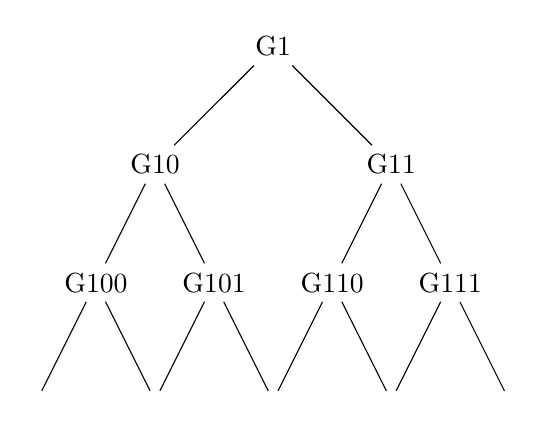
\begin{tikzpicture}[
  level 1/.style={sibling distance=30mm},
  level 2/.style={sibling distance=15mm}
]
  \node {G1}
    child {node {G10}
      child {node {G100}
      child{node{}}
      child{node{}}
      }
      child {node {G101}child{node{}}
      child{node{}}}
    }
    child {node {G11}
      child {node {G110}child{node{}}
      child{node{}}}
      child {node {G111}child{node{}}
      child{node{}}}
    };
\end{tikzpicture}
\end{center}
The height of the tree is log(n).\\
To prove the security of $F$ we can create the following hybrid worlds:
\begin{itemize}
        \item World 0: 
        \begin{itemize}
            \item Challenger chooses $s\leftarrow\{0,1\}^{n}$.
            \item Sends $G'_{log(n)}(\underbrace{G'_{log(n)-1}({\ldots G'_{1}(s)})\ldots})_{\text{log(n) times}}$
            \item A outputs b'.
            \[Pr[A \text{ outputs }0]=p\]
            Here,\[G'_{i}(s1||s2)=\begin{cases}
    G(s1) & \text{ if } x[i]=0 \\
    G(s2) & \text{ if } x[i]=1
\end{cases}\]
        \end{itemize}
        \item Hybrid World i for $0\leq i \leq log(n)$:
        \begin{itemize}
            \item Challenger chooses $r\leftarrow\{0,1\}^{n}$.
            \item Sends $G'_{log(n)}(\underbrace{G'_{log(n)-1}({\ldots G'_{1}(r)})\ldots})_{\text{i times}}$
            \item A outputs b'.
            \[Pr[A \text{ outputs }0]=p_{hi}\]
        \end{itemize}
        \item World 1:
        \begin{itemize}
            \item Challenger chooses $r\leftarrow\{0,1\}^{n}$.
            \item Sends $r$.
            \item A outputs b'.
            \[Pr[A \text{ outputs }0]=p'\]
        \end{itemize}
\end{itemize}
Here, Hybrid world 0 is same as World log(n) and Hybrid World 0 is same as World 1. As the difference between two consecutive hybrid worlds is only of one random and one pseudo random number generated by G, if there exists an adversary which can differentiate between two consecutive hybrid worlds, we can construct a reduction which breaks the security of G. Thus $F$ is secure. 
\subsubsection{}
From the above proof, the probability of differentiating between World 0 and World 1 is at most log(n)*(maximum probability of differentiating between two consecutive hybrid worlds). Thus, if the input space is extended to $\{0,1\}^{n}$, the number of hybrid worlds becomes n and this value becomes n* (maximum probability of differentiating between two consecutive hybrid worlds) which is still negligible. Hence we can say that the proof still works and $F$ is secure.
\subsubsection{}
We can define the following adversary A to break the given PRF construction:
\begin{itemize}
    \item The adversary queries two times, first for $x\leftarrow\{0,1\}^{n}$ and then for $0||x$.
    \item It receives two ciphers $ct00||ct01$ and $ct10||ct11$ respectively.
    \item if $ct10||ct11=G_{n}(ct00)$ then it guesses 0 else guesses 1.
\end{itemize}
The winning probability of this adversary can be calculated by considering the following cases:
\begin{itemize}
    \item the challenger chooses b=0,
    \[Pr[A\text{ guesses }0]=1\]
    \item the challenger chooses b=1,
    \[Pr[A\text{ guesses }1]=1-\frac{1}{2^{n}}\]
\end{itemize}
Thus,
\[Pr[A\text{ wins}]=\frac{1}{2}\cdot\frac{1}{2}+\frac{1}{2}\cdot(1-\frac{1}{2^{n}})=1-\frac{1}{2^{n+1}}\]
Therefore, the adversary A has non negligible advantage.
\subsubsection{}
We can modify the given construction to the following:\\
\\
\fbox{
    \begin{minipage}{\textwidth}
        \centering
        \textbf{PRG → PRF: variable length inputs}\\
        The PRF evaluation using key $k \in \{0,1\}^n$, on input $x \in \{0,1\}^*$ is defined as follows:
        \begin{itemize}
            \item Set $x = k || x$.
            \item Let $s = k$, and let $l$ denote the length of $x$. For $i = 1$ to $l$, do the following:
            \begin{itemize}
                \item Compute $(s_0, s_1) = G^n(s)$, where $s_0$ and $s_1$ are both $n$-bit strings.
                \item Set $s = s_{x[i]}$.
            \end{itemize}
            \item Output $s$.
        \end{itemize}
    \end{minipage}
}
\\
\\
The intuition behind this being secure is that the adversary cannot use attacks using the length of input like the previous attack as the last n operations are unknown which creates exponential possibilities of difference between two inputs in which one is prefix of other. 
\newpage

\section{B.1}
\subsection{CRIME Attack}
\lstinputlisting[language=Python]{attack.py}
The solution takes advantage of the following facts:
\begin{itemize}
    \item If cmsg contains a substring of the cookie, then the compressed string is shorter.
    \item The length of the ‘cookie’ is fixed to be 24 bytes.
\end{itemize}
The attack function tries to recover the secret by iteratively guessing characters of the secret message from left to right. It begins with an empty found string and iterates over each position of the secret string (a total of 24 positions). For each position, the code iterates through all lowercase English letters (from 'a' to 'z') and generates a string by concatenating the characters guessed so far (found) with the current guessed character, followed by a number of spaces to make the total length of the string 24 characters. t then encrypts each constructed string and measures the length of the encrypted output. The length of the encrypted data is used as an indicator of the length of the compressed data, as compression reduces repeated characters. Among all the guesses for the current position, the code selects the character that results in the shortest encrypted length. This choice is made assuming that the character with the shortest encrypted length is more likely to be correct. The guessed character with the minimum encrypted length is appended to the found string. This process continues for all positions in the secret string. After iterating through all positions, the code accumulates the guessed characters into the found string, effectively revealing the secret message character by character.
\newpage
\subsection{Attack on 2DES encryption}
\lstinputlisting[language=Python]{attack_mim.py}
The solution takes advantage of the following facts:
\begin{itemize}
    \item Functions used in both steps are the same(DES).
    \item The key-space is not so large and creating a database for it is feasible.
\end{itemize}
The code iterates over complete key-space using the key\_gen function. 
For each key, the code encrypts the provided message using that key. The encrypted result (e) is used as a key to index the txt1 dictionary, storing the corresponding encryption key for that encrypted result. The code also attempts to decrypt the provided ciphertext using each key.
The decrypted result (d) is used as a key to index the txt2 dictionary, storing the corresponding decryption key for that decrypted result. If a match is found between an encrypted result (e) and a previously stored decrypted result (d) in the txt1 dictionary, it implies that the message was encrypted using the current key and the key for the decrypted result respectively.
If a match is found between a decrypted result (d) and a previously stored encrypted result (e) in the txt2 dictionary, it implies that the message was encrypted using the key for the encrypted result and the current key respectively. The key insight here is that the code leverages the fact that encryption and decryption are inverse operations. If the same intermediate result is obtained from encryption and decryption operations, it indicates a match between the keys used for 2DES.
\end{document}
